% Script-level flow: which file runs when, and what it reads / writes. Build: figures/build.sh
\documentclass[border=10pt]{standalone}
\usepackage[T1]{fontenc}
\usepackage{helvet}
\renewcommand{\familydefault}{\sfdefault}
\usepackage{tikz}
\usetikzlibrary{positioning,fit,arrows.meta,backgrounds,calc}

\definecolor{shared}{HTML}{3B6EA8}
\definecolor{light}{HTML}{1F8A70}
\definecolor{pro}{HTML}{7A4FB5}
\definecolor{ink}{HTML}{222222}
\definecolor{muted}{HTML}{666666}
\definecolor{filec}{HTML}{8A8A8A}

\tikzset{
  script/.style={draw=#1, line width=0.9pt, rounded corners=3pt, fill=#1!8, align=center,
                 inner sep=5pt, text=ink, font=\small\ttfamily, minimum width=34mm, minimum height=9mm},
  script/.default=shared,
  file/.style={draw=filec, line width=0.6pt, fill=white, align=center, inner sep=3pt,
               text=muted, font=\scriptsize\ttfamily, minimum width=34mm,
               double copy shadow={shadow xshift=1.2pt, shadow yshift=-1.2pt, draw=filec!60}},
  lane/.style={draw=#1!60, dashed, rounded corners=6pt, inner sep=8pt},
  lanelabel/.style={font=\bfseries\small, text=#1},
  stage/.style={font=\bfseries\footnotesize, text=muted},
  arr/.style={-{Stealth[length=5pt]}, line width=0.8pt, draw=ink!65},
  sub/.style={font=\scriptsize, text=muted, align=center},
}
\usetikzlibrary{shadows}

\begin{document}
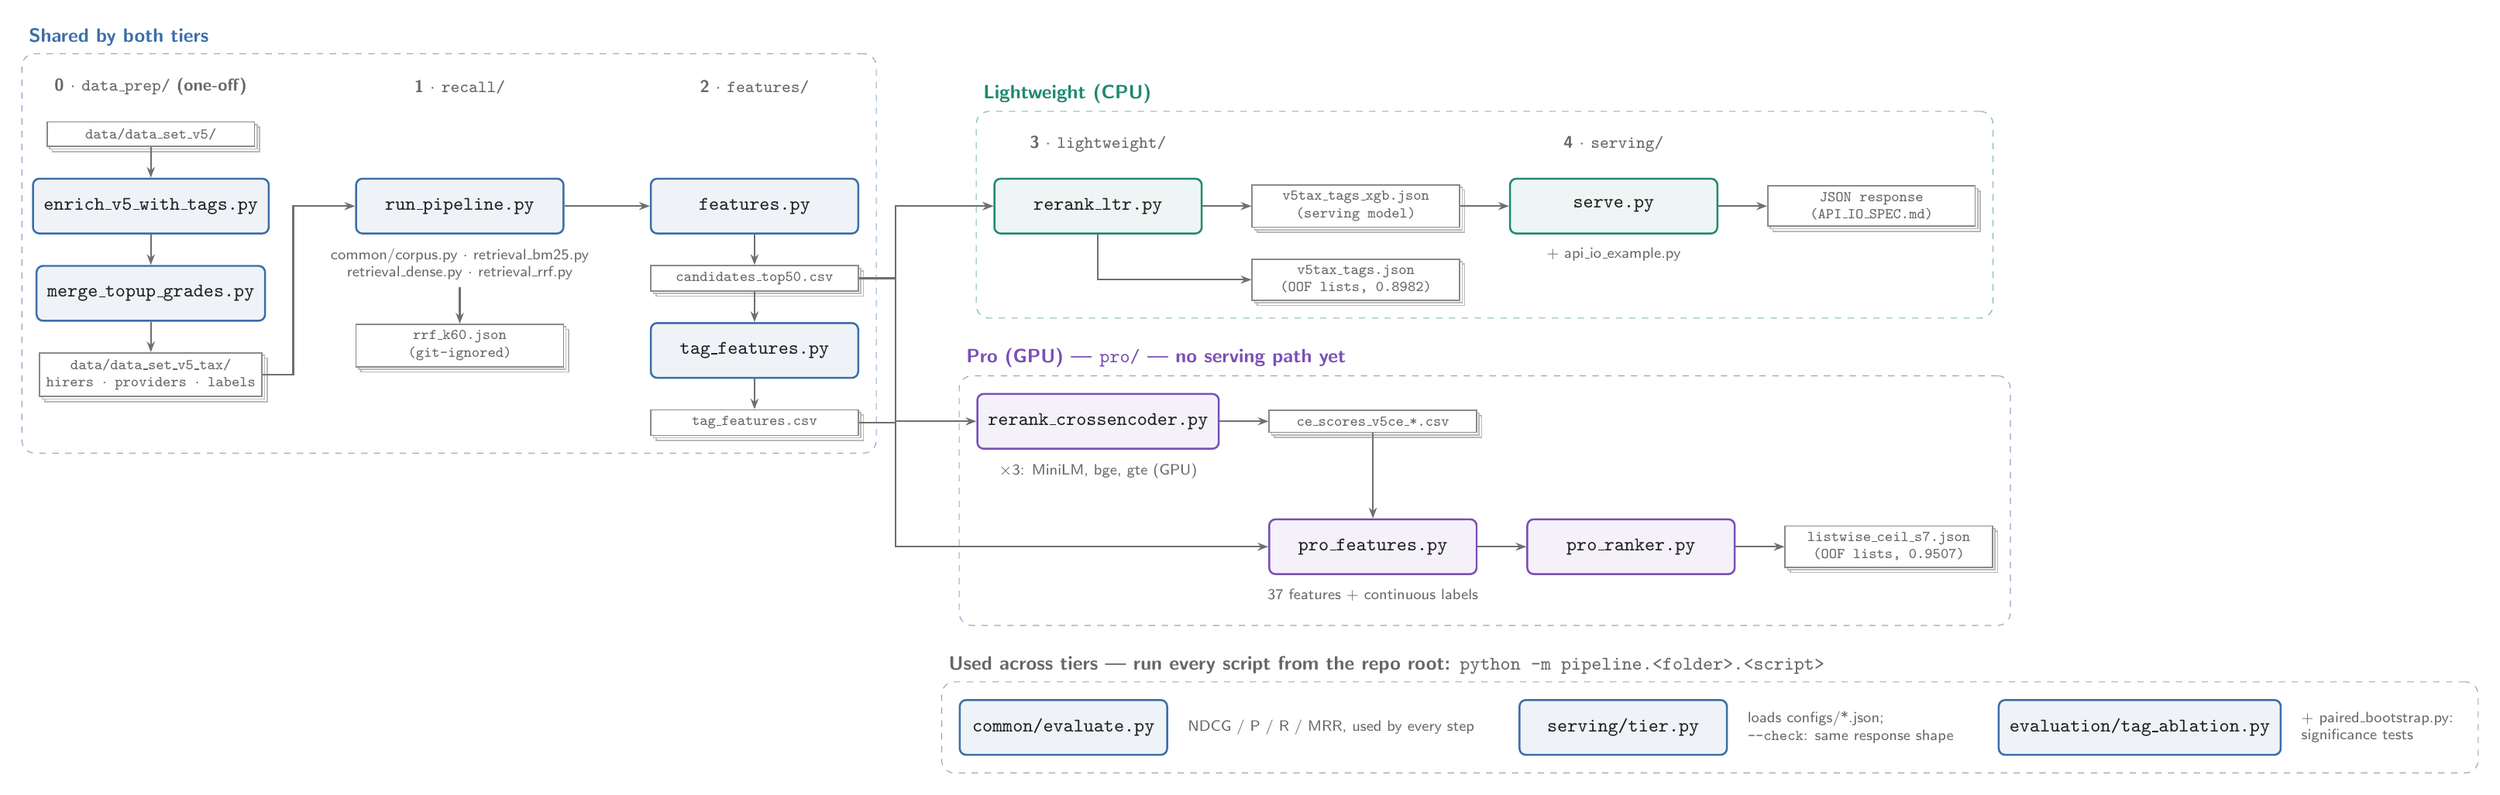
\begin{tikzpicture}[node distance=5mm and 8mm]

% ---------------- 0. data prep ----------------
\node[file] (v5) {data/data\_set\_v5/};
\node[script, below=of v5] (enrich) {enrich\_v5\_with\_tags.py};
\node[script, below=of enrich] (topup) {merge\_topup\_grades.py};
\node[file, below=of topup] (tax) {data/data\_set\_v5\_tax/\\hirers $\cdot$ providers $\cdot$ labels};
\draw[arr] (v5) -- (enrich);
\draw[arr] (enrich) -- (topup);
\draw[arr] (topup) -- (tax);
\node[stage, above=3mm of v5] (s0) {0 $\cdot$ \texttt{data\_prep/} (one-off)};

% ---------------- 1. stage 1 ----------------
\node[script, right=14mm of enrich] (run) {run\_pipeline.py};
\node[sub, below=1mm of run] (runsub) {common/corpus.py $\cdot$ retrieval\_bm25.py\\retrieval\_dense.py $\cdot$ retrieval\_rrf.py};
\node[file, below=6mm of runsub] (rrf) {rrf\_k60.json\\(git-ignored)};
\draw[arr] (tax.east) -- ++(5mm,0) |- (run.west);
\draw[arr] (runsub) -- (rrf);
\node[stage] at (s0 -| run) {1 $\cdot$ \texttt{recall/}};

% ---------------- 2. features ----------------
\node[script, right=14mm of run] (feat) {features.py};
\node[file, below=of feat] (cand) {candidates\_top50.csv};
\node[script, below=of cand] (tagf) {tag\_features.py};
\node[file, below=of tagf] (tagcsv) {tag\_features.csv};
\draw[arr] (run.east) -- (feat.west);
\draw[arr] (feat) -- (cand);
\draw[arr] (cand) -- (tagf);
\draw[arr] (tagf) -- (tagcsv);
\node[stage] at (s0 -| feat) {2 $\cdot$ \texttt{features/}};

\begin{scope}[on background layer]
  \node[lane=shared, fit=(s0)(v5)(tax)(run)(rrf)(feat)(tagcsv)] (sh) {};
\end{scope}
\node[lanelabel=shared, anchor=south west] at (sh.north west) {Shared by both tiers};

% ---------------- 3a. Lightweight ----------------
\node[script=light, right=22mm of feat] (ltr) {rerank\_ltr.py};
\node[file, right=8mm of ltr] (lmodel) {v5tax\_tags\_xgb.json\\(serving model)};
\node[file, below=of lmodel] (loof) {v5tax\_tags.json\\(OOF lists, 0.8982)};
\node[script=light, right=8mm of lmodel] (serve) {serve.py};
\node[sub, below=1mm of serve] {+ api\_io\_example.py};
\node[file, right=8mm of serve] (resp) {JSON response\\(API\_IO\_SPEC.md)};
\draw[arr] (ltr) -- (lmodel);
\draw[arr] (ltr.south) |- (loof.west);
\draw[arr] (lmodel) -- (serve);
\draw[arr] (serve) -- (resp);
\node[stage, above=3mm of ltr] (s3) {3 $\cdot$ \texttt{lightweight/}};
\node[stage] at (s3 -| serve) {4 $\cdot$ \texttt{serving/}};
\begin{scope}[on background layer]
  \node[lane=light, fit=(s3)(ltr)(lmodel)(loof)(serve)(resp)] (lw) {};
\end{scope}
\node[lanelabel=light, anchor=south west] at (lw.north west) {Lightweight (CPU)};

% ---------------- 3b. Pro ----------------
\node[script=pro, below=26mm of ltr] (ce) {rerank\_crossencoder.py};
\node[sub, below=1mm of ce] (cesub) {$\times$3: MiniLM, bge, gte (GPU)};
\node[file, right=8mm of ce] (cecsv) {ce\_scores\_v5ce\_*.csv};
\node[script=pro, below=14mm of cecsv] (pfeat) {pro\_features.py};
\node[sub, below=1mm of pfeat] (pfsub) {37 features + continuous labels};
\node[script=pro, right=8mm of pfeat] (pr) {pro\_ranker.py};
\node[file, right=8mm of pr] (poof) {listwise\_ceil\_s7.json\\(OOF lists, 0.9507)};
\draw[arr] (ce) -- (cecsv);
\draw[arr] (cecsv) -- (pfeat);
\draw[arr] (pfeat) -- (pr);
\draw[arr] (pr) -- (poof);
\begin{scope}[on background layer]
  \node[lane=pro, fit=(ce)(cesub)(cecsv)(pfeat)(pfsub)(pr)(poof)] (pl) {};
\end{scope}
\node[lanelabel=pro, anchor=south west] at (pl.north west) {Pro (GPU) --- \texttt{pro/} --- no serving path yet};

% feature tables feed both tiers
\draw[arr] (cand.east) -- ++(6mm,0) |- (ltr.west);
\draw[arr] (tagcsv.east) -- ++(6mm,0) |- (ltr.west);
\draw[arr] (tagcsv.east) -- ++(6mm,0) |- (ce.west);
\draw[arr] (tagcsv.east) -- ++(6mm,0) |- (pfeat.west);

% ---------------- cross-cutting ----------------
\node[script, below=12mm of pl.south west, anchor=north west] (eval) {common/evaluate.py};
\node[sub, right=2mm of eval, anchor=west, align=left] (evsub) {NDCG / P / R / MRR, used by every step};
\node[script, right=6mm of evsub] (tier) {serving/tier.py};
\node[sub, right=2mm of tier, anchor=west, align=left] (tsub) {loads configs/*.json;\\\texttt{-{}-check}: same response shape};
\node[script, right=6mm of tsub] (abl) {evaluation/tag\_ablation.py};
\node[sub, right=2mm of abl, anchor=west, align=left] (asub) {+ paired\_bootstrap.py:\\significance tests};
\begin{scope}[on background layer]
  \node[lane=muted, fit=(eval)(evsub)(tier)(tsub)(abl)(asub)] (cc) {};
\end{scope}
\node[lanelabel=muted, anchor=south west] at (cc.north west) {Used across tiers --- run every script from the repo root: \texttt{python -m pipeline.<folder>.<script>}};

\end{tikzpicture}
\end{document}
